\vspace{-10pt}
\section{Evaluation}\label{sec:evaluation}
The evaluation of our preemption point placement algorithm will embody
two methods: 1) characterization and measurement of preemption costs
using real-time application code, and 2) a breakdown utilization schedulability
comparison for various CRPD computational approaches.
%2) a schedulability comparison
%of synthetic task set for various preemption models.
%\vspace{-10pt}
\subsection {Preemption Cost
  Characterization}\label{sec:preemption_cost_measurement}
To characterize the behavior and estimate the benefit of the approach
proposed in this paper, a case study of representative tasks was
performed. The tasks were selected from the Malardalen University (MRTC) WCET benchmark suite~\cite{mrtc:01}. Each task was built using Gaisler's Bare-C Cross Compiler~\cite{gaisler:01} for the GRSIM LEON3~\cite{gaisler:02} simulated target.
%
%During execution of a task within a specific basic block, variance in the number of shared
%UCBs between program points is related to the execution flow of the task through each of
%the points. For instance, one path to program point ${\varrho_i^j}$ may include only ${\varrho_i^h}$,
%while another path to ${\varrho_i^j}$ may contain ${\varrho_i^h}$ followed by
%${\varrho_i^m}$. The set of UCBs shared between ${\varrho_i^h}$ and ${\varrho_i^j}$ may differ
%based on the path between them. If the paths differ one of them may
%result in a greater number of shared UCBs between the points. To
%accurately upper-bound the shared UCBs between points requires
%complete control flow information.

Tasks were first analyzed using AbsInt's a\textsuperscript{3} WCET~\cite{absint:01}
to determine the set of basic blocks. Next, the basic blocks ${\{\delta_i^1, \delta_i^2, ..., \delta_i^{N_i}\}}$ were serialized by recording their order during execution. Program points were identified as the address of the final instruction of each basic block ${\delta_i^j}$ for $j \in [0, N_i]$ to match the sequential basic block structure used by our preemption point placement algorithm. Each program point served as a breakpoint when running the task on the simulator. In accordance with the sequential basic block structure used in our algorithm, only the data cache is used to compute CRPD as the linear basic block structure offers only limited opportunities for instruction cache blocks to be revisited.

During the execution of each basic block, the data cache states were saved as ${\Upsilon_D(\delta_i^j)}$ at each breakpoint. As expected, the data cache contents were highly dependent on the actual basic block instruction control flow during execution.  The cache snapshots were selected as the final visit of each program point where the data cache contents ${\Upsilon_D(\delta_i^j)}$ were captured, and recorded. From the final ${\Upsilon_D(\delta_i^j)}$ snapshots, a conservative estimate of LCBs shared between program points was determined.
%Given the limitations of the simulator and a\textsuperscript{3} it was not possible to record the actual control flow.
%Thus, calculating an accurate over-estimate of the LCBs shared between program points was not possible. A %selection of cache snapshots were chosen as an estimation of the actual cache behavior.
%
%A program point ${\varrho_i^j}$ may be visited multiple
%times during a tasks execution. The UCBs shared between ${\varrho_i^j}$ and a
%later point ${\varrho_i^k}$ could change with each visit of ${\varrho_i^j}$. During
%the final visit of ${\varrho_i^j}$ the instruction and data cache contents
%were captured, and recorded as ${\Upsilon_I(\delta_i^j)}$ and ${\Upsilon_D(\delta_i^j)}$.
%From these representative snapshots, a representative over-estimate of shared
%UCBs were made.

Shared LCBs were calculated by intersecting the cache state snapshots from ${\delta_i^j}$
to ${\delta_i^k}$, except ${\delta_i^k}$. A cache line that remains unchanged after
the execution of $\{{\delta_i^j}$, ${\delta_i^{j+1}}$, ..., ${\delta_i^{k-1}}\}$ will be present in the cache before execution of the basic block that ${\delta_i^k}$ represents. It is only from these unchanged cache lines that the shared LCBs between ${\delta_i^j}$ and ${\delta_i^k}$ can be selected. The complete set of
unchanged cache lines serves as a safe upper-bound on the LCBs shared between each basic block pair. The equation below formalizes this idea, using the data cache snapshots ${\Upsilon_D(\delta_i^j)}$.
\vspace{-20pt}
\begin{center}
  \begin{equation}
    LCB(\delta_i^j,\delta_i^k) \subseteq \bigcap_{m=j}^{k-1} {\Upsilon_D(\delta_i^m)}
  \end{equation}
\end{center}
\subsubsection{Availability}
This method may be verified and reproduced using the same tools and data. Gaisler's compiler and simulator are freely available. AbsInt's a\textsuperscript{3} tool is available for educational and evaluation purposes. The programs written and data used in this paper can be found on GitHub~\cite{tessler:14} thereby permitting the research community to reproduce and leverage our work as needed.
\newline
\subsubsection{Results}
The results are presented as a comparison between our proposed method and the Bertogna method\cite{bertogna:11}, which uses a single value for CRPD at each program point.  In terms of LCB computation this implies that the maximum LCB value over all subsequent program points must be used as the CRPD cost:
\begin{equation}
  \max\{LCB(\delta_i^j,\delta_i^k)\ \vert\ j\ <\ k\}
\end{equation}
%
%To determine the maximum benefit of the new approach, the best case
%scenario is considered. When the preemption point is selected with the
%fewest number of UCBs based upon previous preemption.  For ${\varrho_i^j}$ the
%determination is made by:
%\begin{equation*}
%  \min\{ UCB(\varrho_i^j, \varrho_i^k) \vert j < k \}
%\end{equation*}

In the following graphs, each point in the graph represents two points in the program. The first point of the program ${\delta_i^j}$ is fixed by the x-axis. The y-axis indicates the shared LCB count with a later program
point. The first graph, representing the recursion benchmark task data cache in Figure~\ref{fig:recusion_data_cache}, shows the minimum and maximum shared LCBs between various program
points. At each point on the graph, the index of the next preemption point associated with the respective minimum or maximum graph value at that location is shown.  At program point ${\delta_i^4}$, the minimum CRPD value is coupled with program point ${\delta_i^7}$ having a shared LCB count of 14 whereas the single valued CRPD computation method finds 24 shared LCBs coupled at program point ${\delta_i^5}$.
%
\begin{figure}[h!]
\vspace{-10pt}
\begin{center}
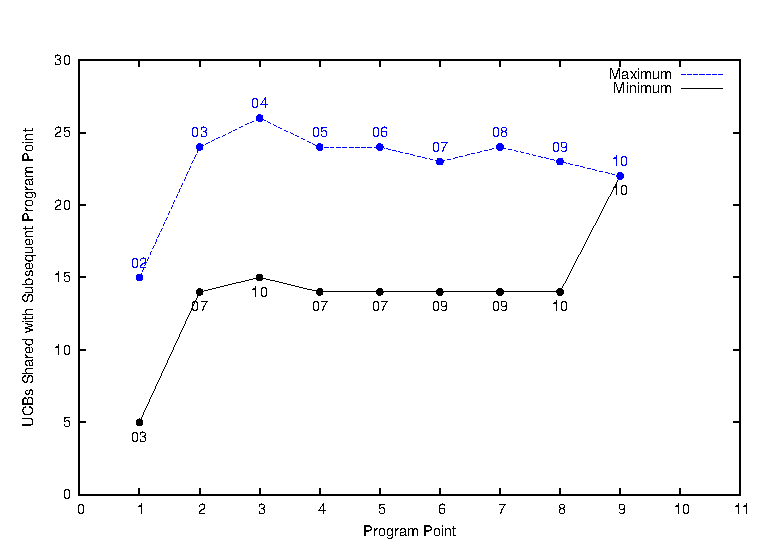
\includegraphics[width=\linewidth]{eps/recursion-dcache.eps}
\caption{Recursion Data Cache.}
\label{fig:recusion_data_cache}
\end{center}
\vspace{-10pt}
\end{figure}

To compare the two preemption point placement algorithms their selection of two program points is
simulated by assuming ${Q_i}$ is larger than the task's total execution time. Bertogna's algorithm would select the preemption point commensurate with the lowest value of the dashed line. Our algorithm would select the preemption point commensurate with the lowest value of the solid line.  The difference between the performance of these two preemption point placement algorithms is an example of the benefit provided by considering location aware CRPD cost.

The second graph represents the lms benchmark task data cache shown in Figure~\ref{fig:lms_data_cache}, and the third graph represents the adpcm benchmark task data cache shown in Figure~\ref{fig:adpcm_data_cache}. Similar to the recursion benchmark data cache, the variability in the minimum and maximum shared LCBs for each program point further exemplifies the benefit of using location aware CRPD cost in preemption point placement.  Maximum and minimum data cache costs for the other seven tasks show similar variability but are not shown here due to space limitations.
\begin{figure}[h!]
\vspace{-10pt}
\begin{center}
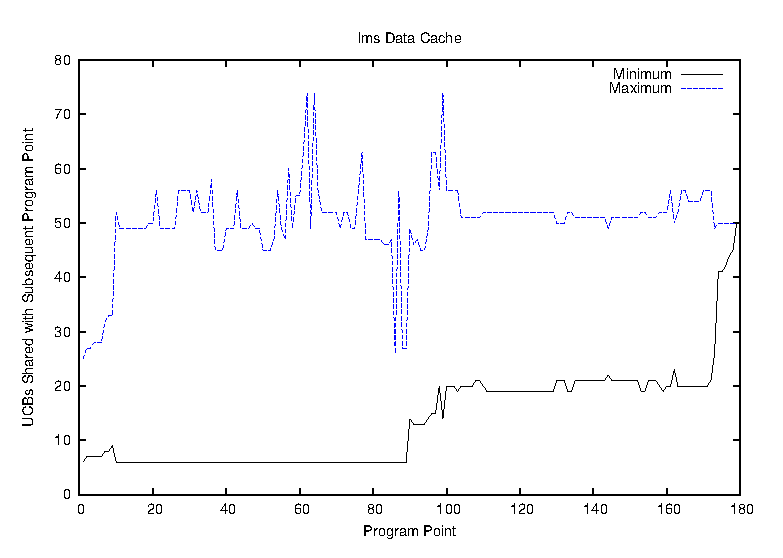
\includegraphics[width=\linewidth]{eps/lms-dcache.eps}
\caption{LMS Data Cache.}
\label{fig:lms_data_cache}
\end{center}
\vspace{-10pt}
\end{figure}
%\vspace{-20pt}
\begin{figure}[h!]
\vspace{-10pt}
\begin{center}
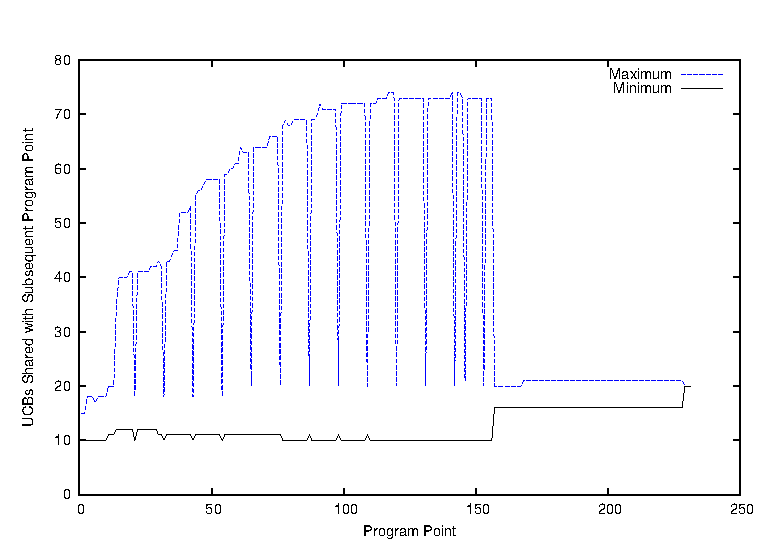
\includegraphics[width=\linewidth]{eps/adpcm-dcache.eps}
\caption{ADPCM Data Cache.}
\label{fig:adpcm_data_cache}
\end{center}
\vspace{-10pt}
\end{figure}
%
%\begin{table}[h!]
%%{\fontsize{10}{10}\selectfont
%\small
%\begin{minipage}{\linewidth}
%\centering
%    \begin{tabular}{l | l | l || l | l | l}
%      Task & Cache & Benefit & Task & Cache & Benefit\\
%      \hline
%
%      adpcm & ${I}$ & 143 & fft1 & ${I}$ & 72 \\
%            & ${D}$ & 5 & & ${D}$ & 13\\
%      \hline
%
%      bsort & ${I}$ & 0 & fibcall & ${I}$ & 1 \\
%            & ${D}$ & 0 & & ${D}$ & 1 \\
%      \hline
%
%      cnt & ${I}$ & 63 & lms & ${I}$ & 158 \\
%          & ${D}$ & 2 & & ${D}$ & 18 \\
%      \hline
%
%      cover & ${I}$ & 135 & ndes & ${I}$ & 96 \\
%            & ${D}$ & 2 & & ${D}$ & 15 \\
%      \hline
%
%      crc & ${I}$ & 18 & recursion & ${I}$ & 7 \\
%          & ${D}$ & 1 & & ${D}$ & 10  \\
%      \hline
%
%    \end{tabular}
%    \bigskip
%    \caption {Benefit of Proposed Method}
%    \label{tab:proposed_method_benefit}
%
%    Benefit of Proposed Method
%    \bigskip
%\end{minipage}
%\normalsize
%}
%\vspace{-20pt}
%\end{table}
%
%\begin{minipage}{\linewidth}
%\centering
%  \caption {Benefit of Proposed Method}
%    \begin{tabular}{l l | l}
%      Task & Cache & Benefit \\
%      \hline
%
%      adpcm & ${I}$ & 143 \\
%            & ${D}$ & 5 \\
%      \hline
%
%      bsort & ${I}$ & 0 \\
%            & ${D}$ & 0 \\
%      \hline
%
%      cnt & ${I}$ & 63 \\
%          & ${D}$ & 2 \\
%      \hline
%
%      cover & ${I}$ & 135 \\
%            & ${D}$ & 2 \\
%      \hline
%
%      crc & ${I}$ & 18 \\
%          & ${D}$ & 1 \\
%      \hline
%
%      fft1 & ${I}$ & 72 \\
%           & ${D}$ & 13 \\
%      \hline
%
%      fibcall & ${I}$ & 1 \\
%              & ${D}$ & 1 \\
%      \hline
%
%      lms & ${I}$ & 158 \\
%          & ${D}$ & 18 \\
%      \hline
%
%      ndes & ${I}$ & 96 \\
%           & ${D}$ & 15 \\
%      \hline
%
%      recursion & ${I}$ & 7 \\
%                & ${D}$ & 10 \\
%      \hline
%
%    \end{tabular}
%    \bigskip
%
%    Benefit of Proposed Method
%    \bigskip
%\end{minipage}

In examining the graphs for all tasks and data caches a few common traits were noted. The minimum shared LCBs sharply increases at the end of each task's execution. This is due to the nature of the conservative estimation of shared LCBs and the tasks, and the number of instructions in the basic block between the final program points is relatively small thereby limiting the number of data cache lines that could be eliminated by the intersection.
%
%This behavior limits the appropriate type of analysis. The preceding table shows the maximum benefit of the proposed approach. If the minimum benefit %were considered it would always be zero; since the difference in estimated shared LCBs converges at the final basic block.

Drastic spikes downwards in the shared LCB counts for the minimum and maximum curves coincide with function call boundaries, or large conditional blocks. At these boundaries, the maximum and minimum LCB counts are approximately the same. There is a sharp upward spike in the early program points for the maximum curves. This trend is due to the early initialization blocks built into tasks. In our analysis, the minimum curves show a clear benefit of selecting preemption points outside of the early initialization section.
%This may be an area for further study, using a greater number of tasks.
\vspace{-10pt}
\subsection{Breakdown Utilization}
The previous analysis illustrates the benefit of using location aware CRPD cost in preemption point placement thereby reducing the preemption overhead
for an individual task, however, it does not address the benefits to task set schedulability. To evaluate task set schedulability benefits a second case study was performed focusing on the breakdown utilization of the MRTC WCET benchmark suite~\cite{mrtc:01} for various algorithms.  Our study compares the Luniss et. al. UCB only approach for EDF~\cite{lunniss:13}, the Bertogna et. al. Explicit Preemption Point Placement algorithm~\cite{bertogna:11}, and our improved Explicit Preemption Point Placement algorithm. For notational convenience the UCB Only approach for EDF will be referred to as ${UOE}$, the Bertogna Explicit Preemption Point Placement algorithm as ${BEPP}$, and our Explicit Preemption Point Placement algorithm as ${EPP}$.

The appropriate schedulablity test for ${UOE}$ is comprised of three parts: ${\gamma^{ucb}_{t,j}}$, ${U^*_j}$, and ${U^*}$ each representing
the maximum CRPD for task \begin{math}\tau_{j}\end{math}, the utilization of task \begin{math}\tau_{j}\end{math} including CRPD, and the utilization of the task set
respectively as documented in Lunniss \emph{et~al.}~\cite{lunniss:13}. A task set is schedulable when ${U^* \le 1}$.
%
%The appropriate schedulablity test for ${UOE}$ is found in
%Lunniss \emph{et~al.}~\cite{lunniss:13}. It is comprised of three
%parts: ${\gamma^{ucb}_{t,j}}$, ${U^*_j}$, and ${U^*}$. They represent
%the maximum CRPD for a task ${j}$, the utilization of the task ${j}$
%including the CRPD of the task, and the utilization of the task set.
%A task set is schedulable when ${U^* \le 1}$.
%\begin{equation}
%  \gamma^{ucb}_{t,j} = BRT \cdot \max\limits_{\forall k \in aff(t,j)}
%  \left\{ \left| UCB_k \right| \right\}
%\end{equation}
%\begin{equation}
%  U^*_j = \frac{C_j + \gamma^{ucb}_{t,j}}{T_j}
%\end{equation}
%\begin{equation}
%  U^* = \sum^{N}_{j=1} U^*_j
%\end{equation}
%where $aff(t,j)$ is the set of tasks that can be preempted by jobs of
%task $\tau_{i}$ in an interval of length t~\cite{lunniss:13} as shown below.
%\begin{equation}
%  aff(t,j) = \{\forall\ \tau_{i}\ |\ t\ \geq D_{i} > D_{j}\}
%\end{equation}
\newline
\indent
%\begin{equation}
%  \gamma^{ucb}_j = BRT \cdot \max\limits_{k \in \tau}
%  \left\{ \left| UCB_k \right| \right\}
%\end{equation}
%\begin{equation}
%  U^*_j = \frac{C_j + \gamma^{ucb}_j}{T_j}
%\end{equation}
%\begin{equation}
%  U^* = \sum_{i \in \tau} U^*_i
%\end{equation}
%
%The task set from which the breakdown utilization benefit is
%calculated comes, again, from the MRTC suite \cite{mrtc:01}.
Borrowing the breakdown utilization evaluation technique from \cite{lunniss:13}, each task has its deadline and period set to ${T_i = P_i = u \cdot C_i}$ where ${u}$ is a constant. The constant, ${u}$, begins at the number of tasks (ten) and is increased in steps of 0.25 until the task set becomes schedulable. Incremental negative adjustments are then made to determine when the set becomes unschedulable, indicating the final breakdown utilization.
%
%The final parameter, ${UCB_k}$ is obtained by modifying the earlier
%evaluation section \emph{Preemption Cost Characterization}.
For each task, the set of shared LCBs are calculated at each program point. Taking the maximum shared LCB count for any task is safe and appropriate for calculating ${U^*}$.

For ${BEPP}$, the maximum shared LCB counts obtained in the earlier evaluation serve as input. Lastly, for ${EPP}$, the shared LCB counts obtained in the earlier evaluation serve as input for our Explicit Preemption Point Placement algorithm.  The last input variables required for both approaches are ${C_i}$ and ${BRT}$. ${C_i}$ was captured as the total number of cycles required to complete the task without preemptions. The breakdown utilization study sweeps the ${BRT}$ parameter from 10 ${{\mu}s}$ to 390 ${{\mu}s}$, representing values across several different types of processors.

The breakdown utilization determination leverages our iterative schedulability and preemption point placement algorithm as outlined in the following steps below as given in Algorithm~\ref{alg:iterative-breakdown-utilization-algo}.
%{\fontsize{10}{10}\selectfont
\begin{algorithm}
\caption{Breakdown Utilization Evaluation Algorithm}
\label{alg:iterative-breakdown-utilization-algo}
\begin{algorithmic}[1]
\small
\State{Start with a task system that may or may not be feasible.}
\State{Assume the CRPD of the task system is initially zero.}
\Repeat
   \State\begin{varwidth}[t]{\linewidth}
    Run the Iterative Schedulability and Preemption Point Placement Algorithm \ref{alg:iterative-schedulability-optimal-ppp} \par
    \end{varwidth}
%
%    \Repeat
%        \State\begin{varwidth}[t]{\linewidth}
%        Run the Baruah algorithm to obtain the maximum \par
%        \hskip\algorithmicindent non-preemptive region $Q_i$ for each task.
%        \end{varwidth}
%        \State\begin{varwidth}[t]{\linewidth}
%        Select optimal preemption points using our \par
%        \hskip\algorithmicindent dynamic programming algorithm.
%        \end{varwidth}
%        \State\begin{varwidth}[t]{\linewidth}
%        Compute the CRPD and the preemptive WCET \par
%        \hskip\algorithmicindent $C_i$ from the selected preemption points.
%        \end{varwidth}
%    \Until{the selected preemption points do not change.}
%
    \If{the task system is feasible/schedulable}
        \State\begin{varwidth}[t]{\linewidth}
        Increase the system utilization by decreasing the \par
        \hskip\algorithmicindent periods via a binary search.
        \end{varwidth}
    \Else
        \State\begin{varwidth}[t]{\linewidth}
        Decrease the system utilization by increasing the \par
        \hskip\algorithmicindent periods via a binary search.
        \end{varwidth}
    \EndIf
\Until\begin{varwidth}[t]{\linewidth}
the utilization change is less than some tolerance.
\end{varwidth}
\State{The breakdown utilization is given by U.}
\normalsize
\end{algorithmic}
\end{algorithm}
%}
Using ten tasks, the breakdown utilization comparison between ${UOE}$, ${BEPP}$, and ${EPP}$ are summarized in Figure~\ref{fig:breakdown_utilization}.
\begin{figure}[h!]
\vspace{-10pt}
\begin{center}
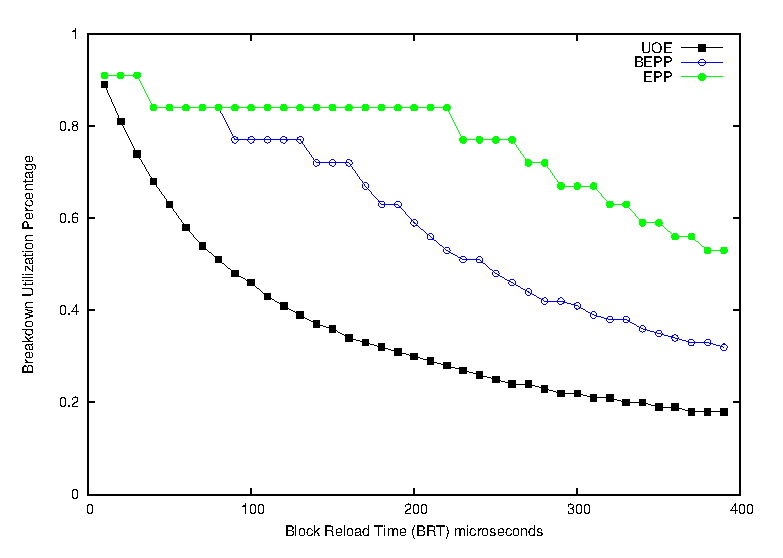
\includegraphics[width=\linewidth]{eps/breakdown.eps}
\caption{Breakdown Utilization Comparison.}
\label{fig:breakdown_utilization}
\end{center}
\vspace{-10pt}
\end{figure}
%\begin{table}[h!]
%\small
%\begin{minipage}{\linewidth}
%\vspace{-20pt}
%  \bigskip
%  \centering
%    \begin{tabular}{c | c}
%      Method & Utilization \\
%      \hline
%      UOE & .29 \\
%      EPP & TBD \\
%    \end{tabular}
%    \bigskip
%    \caption {Breakdown Utilization Summary}
%    \label{tab:breakdown_utilization_summary}
%\normalsize
%\end{minipage}
%\normalsize
%\vspace{-20pt}
%\end{table}
The breakdown utilization results indicate that $BEPP$ dominates the $UOE$ algorithm primarily due to the limited preemption model utilizing CRPD cost at the basic block level.  $EPP$ dominates $BEPP$ resulting from the more accurate location aware CRPD cost used in our preemption point placement algorithm.  As expected, the breakdown utilization converges for all three methods convergence for small ${BRT}$ values.
%Compared to \cite{lunniss:13} this evaluation of ${UOE}$ has an average breakdown utilization approximately 17\% lower. This is likely due to a %different selection of benchmark tasks and our subsequent estimation technique used for computing the set of UCBs. The data used in \cite{lunniss:13} %does not include UCB information per basic block, which is required for ${BEPP}$ and ${EPP}$, thereby necessitating the generation of new LCB estimates %for each task.
%
%\clearpage
%
%\subsection {Taskset Schedulability Evaluation}\label{sec:taskset schedulability}
%The schedulability performance metrics we intend to compare various
%preemption models with are: 1) the percentage of schedulable task sets
%as a function of the task set utilization, 2) the percentage of
%schedulable task sets as a function of the number of tasks, 3) the
%percentage of schedulable task sets as a function of the maximum CRPD,
%and 4) the percentage of schedulable task sets as a function of the
%variability of the CRPD variance \begin{math}\sigma_{CRPD}\end{math}.
%The following preemption models will be studied namely: 1) fully
%non-preemptive, 2) fully preemptive, 3) limited preemption naive
%approach, 4) limited preemption point placement with fixed CRPD
%preemption cost, 5) limited preemption point placement with variable
%CRPD preemption cost, and 6) optimal preemption point placement with
%enhanced CRPD preemption cost.
%
%Our approach for generating the synthetic task sets involves a number
%of steps which is summarized as follows.  The number of basic blocks
%generated each task is in the
%interval \begin{math}[N_{i}(min),N_{i}(max)]\end{math} using a random
%uniform distribution.  Each basic block non-preemptive WCET is
%generated using a Gaussian distribution with
%mean \begin{math}\mu_{WCET}\end{math} and
%variance \begin{math}\sigma_{WCET}\end{math}.  The  utilization of
%each task has been generated using the approach proposed in [TBD12].
%The task periods \begin{math}T_{i}\end{math} were then computed
%dividing the non-preemptive WCET \begin{math}C_{i}^{NP}\end{math} by
%the utilization \begin{math}U_{i}\end{math} of each task.  Preemption
%costs were randomly generated using the following function (TBD), to
%achieve a realistic distribution similar to the one derived
%empirically).  The enhanced CRPD is generated to be a percentage of
%the WCET in the interval [0, 0.50] with a random uniform
%distribution. Cache related preemption delay (CRPD) values are
%generated for each pair of potential preemption points.  The variable
%CRPD preemption cost model uses the CRPD cost from the each preemption
%point to the end of the task. The fixed CRPD preemption cost model
%uses the maximum CRPD cost of all variable CRPD preemption cost
%values. 